\documentclass[12pt,a4paper]{article}
\usepackage[utf8]{inputenc}
\usepackage[french]{babel}
\usepackage[T1]{fontenc}
\usepackage{amsmath}
\usepackage{amsfonts}
\usepackage{amssymb}
\usepackage{graphicx}
\usepackage[left=2cm,right=2cm,top=3cm,bottom=2cm]{geometry}
\usepackage{multicol}
\usepackage[thinspace,thinqspace,amssymb]{SIunits}
\usepackage{pifont}
\usepackage{tikz}
\usepackage{multicol}
\usepackage{fourier}
\usepackage{setspace}
\usepackage{enumitem}

\usepackage{url}
\usepackage[breaklinks]{hyperref}
\hypersetup{
    colorlinks=true,
    linkcolor=red_f,
    citecolor=bleu_f,
    filecolor=green_f,
    urlcolor=bleu_f
}
\usepackage[hyphenbreaks]{breakurl}

\renewcommand{\familydefault}{\sfdefault}

\usepackage{xcolor}
\definecolor{gray_f}{RGB}{68,84,106}
\definecolor{gray_c}{RGB}{214,220,229}
\definecolor{bleu_f}{RGB}{91,155,213}
\definecolor{bleu_c}{RGB}{222,235,247}
\definecolor{red_f}{RGB}{204,0,0}
\definecolor{red_c}{RGB}{245,204,204}
\definecolor{orange_f}{RGB}{237,125,49}
\definecolor{orange_c}{RGB}{251,229,214}
\definecolor{green_f}{RGB}{112,173,71}
\definecolor{green_c}{RGB}{226,240,217}
\definecolor{yellow_f}{RGB}{255,192,0}
\definecolor{yellow_c}{RGB}{255,242,204}

\usepackage{fancyhdr}
\pagestyle{fancy}
\lhead{\textcolor{gray_f}{Physique-Chimie\\R. METZDORFF}}
\chead{\textcolor{gray_f}{Lycée Suzanne Valadon}}
\rhead{\textcolor{gray_f}{2020-2021}}
\renewcommand{\headrulewidth}{0.4pt}
\let\HeadRule\headrule
\renewcommand\headrule{\color{gray_f}\HeadRule}

%%%%% New environnements
\usepackage[framemethod=tikz]{mdframed}
\usepackage{chngcntr}

%%% header
\mdfdefinestyle{s_head}{%
	linecolor=gray_f!,
	outerlinewidth=3pt,%
	frametitlerule=false,
	topline=false,
	bottomline=false,
	rightline=false,
	leftline=false,
	backgroundcolor=gray_c,
	innertopmargin=8pt,
	roundcorner=0pt,
	nobreak=true,
	fontcolor=gray_f
}
\newmdenv[style=s_head]{header_env}
\newenvironment{header}
{%\stepcounter{exa}%
	\addcontentsline{ldf}{figure}{0}%
	\begin{header_env}\centering\LARGE\bf}
	{\end{header_env}}
	
%%% definition
\mdfdefinestyle{s_def}{%
	linecolor=red_f!,
	outerlinewidth=3pt,%
	frametitlerule=false,
	topline=false,
	bottomline=false,
	rightline=false,
	leftline=true,
	backgroundcolor=red_c,
	innertopmargin=8pt,
	roundcorner=0pt,
	nobreak=true,
	fontcolor=red_f
}
\newmdenv[style=s_def]{def_env}
\newenvironment{definition}
{%\stepcounter{exa}%
	\addcontentsline{ldf}{figure}{0}%
	\begin{def_env}\textbf{Définition :}}
	{\end{def_env}}

%%% exemple
\mdfdefinestyle{s_ex}{%
	linecolor=gray_f!,
	outerlinewidth=3pt,%
	frametitlerule=false,
	topline=false,
	bottomline=false,
	rightline=false,
	leftline=true,
	backgroundcolor=gray_c,
	innertopmargin=8pt,
	roundcorner=0pt,
	nobreak=true,
	fontcolor=gray_f
}
\newmdenv[style=s_ex]{ex_env}
\newenvironment{exemple}
{%\stepcounter{exa}%
	\addcontentsline{ldf}{figure}{0}%
	\begin{ex_env}\textbf{Exemple :}}
	{\end{ex_env}}

%%% analyse a priori
\mdfdefinestyle{s_prior}{%
	linecolor=green_f!,
	outerlinewidth=3pt,%
	frametitlerule=false,
	topline=false,
	bottomline=false,
	rightline=false,
	leftline=true,
	backgroundcolor=green_c,
	innertopmargin=8pt,
	roundcorner=0pt,
	nobreak=true,
	fontcolor=green_f
}
\newmdenv[style=s_prior]{prior_env}
\newenvironment{prior}
{%\stepcounter{exa}%
	\addcontentsline{ldf}{figure}{0}%
	\begin{prior_env}\textbf{A priori :}}
	{\end{prior_env}}

%%% analyse a posteriori
\mdfdefinestyle{s_post}{%
	linecolor=green_f!,
	outerlinewidth=3pt,%
	frametitlerule=false,
	topline=false,
	bottomline=false,
	rightline=false,
	leftline=true,
	backgroundcolor=green_c,
	innertopmargin=8pt,
	roundcorner=0pt,
	nobreak=true,
	fontcolor=green_f
}
\newmdenv[style=s_post]{post_env}
\newenvironment{post}
{%\stepcounter{exa}%
	\addcontentsline{ldf}{figure}{0}%
	\begin{post_env}\textbf{A posteriori :}}
	{\end{post_env}}
	
%%% Experience

\mdfdefinestyle{s_experience}{%
	linecolor=bleu_f!,
	outerlinewidth=3pt,%
	frametitlerule=false,
	topline=false,
	bottomline=false,
	rightline=false,
	backgroundcolor=bleu_c,
	innertopmargin=8pt,
	roundcorner=0pt,
	nobreak=true
}
\newmdenv[style=s_experience]{experience_env}
\newenvironment{experience}
{%\stepcounter{exa}%
	\addcontentsline{ldf}{figure}{0}%
	\begin{experience_env}}
%	\begin{experience_env}[]{\noindent\colorbox[rgb]{0.1 0.1 0.53}{\textbf{\color{white} Expérience : }}\\}}
	{\end{experience_env}}

%%% Slide

\mdfdefinestyle{s_slide}{%
	linecolor=green_f!,
	outerlinewidth=3pt,%
	frametitlerule=false,
	topline=false,
	bottomline=false,
	rightline=false,
	backgroundcolor=green_c,
	innertopmargin=8pt,
	roundcorner=0pt,
	nobreak=true
}
\newmdenv[style=s_slide]{slide_env}

\newenvironment{slide}
	{%\stepcounter{exa}%
%		\newenvironment{myenv}{\begin{adjustwidth}{2cm}{}}{\end{adjustwidth}}
		\addcontentsline{ldf}{figure}{0}%
		\begin{slide_env}}
		{\end{slide_env}
	}

%%% Conseils
\mdfdefinestyle{s_conseil}{%
	linecolor=orange_f!,
	outerlinewidth=3pt,%
	frametitlerule=false,
	topline=false,
	bottomline=false,
	rightline=false,
	backgroundcolor=orange_c,
	innertopmargin=8pt,
	roundcorner=0pt,
	nobreak=true,
	fontcolor=orange_f
}
\newmdenv[style=s_conseil]{conseil_env}
\newenvironment{conseil}
{%\stepcounter{exa}%
	\addcontentsline{ldf}{figure}{0}%
	\begin{conseil_env}\textbf{Conseil :}}
	{\end{conseil_env}
	}

%%% Remarque
\mdfdefinestyle{s_remarque}{%
	linecolor=green_f!,
	outerlinewidth=3pt,%
	frametitlerule=false,
	topline=false,
	bottomline=false,
	rightline=false,
	backgroundcolor=green_c,
	innertopmargin=8pt,
	roundcorner=0pt,
	nobreak=true,
	fontcolor=green_f
}
\newmdenv[style=s_remarque]{remarque_env}
\newenvironment{remarque}
{%\stepcounter{exa}%
	\addcontentsline{ldf}{figure}{0}%
	\begin{remarque_env}\textbf{Remarque :}}
	{\end{remarque_env}
	}
	
%%% Document
\mdfdefinestyle{s_doc}{%
	linecolor=bleu_f!,
	outerlinewidth=1pt,%
	frametitlerule=false,
	topline=true,
	bottomline=true,
	rightline=true,
	backgroundcolor=white,
	innertopmargin=8pt,
	roundcorner=0pt,
	nobreak=true,
	fontcolor=black
}
\newmdenv[style=s_doc]{doc_env}
\newenvironment{doc}
{%\stepcounter{exa}%
	\addcontentsline{ldf}{figure}{0}%
	\begin{doc_env}\textbf{Document}}
	{\end{doc_env}
	}
	
%%% Données
\mdfdefinestyle{s_don}{%
	linecolor=bleu_f!,
	outerlinewidth=1pt,%
	frametitlerule=false,
	topline=true,
	bottomline=true,
	rightline=true,
	backgroundcolor=white,
	innertopmargin=8pt,
	roundcorner=0pt,
	nobreak=true,
	fontcolor=black
}
\newmdenv[style=s_don]{don_env}
\newenvironment{donnee}
{%\stepcounter{exa}%
	\addcontentsline{ldf}{figure}{0}%
	\begin{don_env}\textcolor{bleu_f}{\textbf{Données}}}
	{\end{don_env}
	}

%%%%% New command

\newcommand{\diazote}{\text{N}_2}
\newcommand{\dioxygene}{\text{O}_2}
\newcommand{\dioxydedecarbone}{\text{CO}_2}
\newcommand{\eau}{\text{H}_2\text{O}}
\newcommand{\chlorure}{\text{Cl}^-}
\newcommand{\prof}[1]{\textcolor{gray_f}{\textit{#1}}}

\newcommand{\app}{\colorbox{bleu_c}{\textcolor{bleu_f}{APP}}}
\newcommand{\rea}{\colorbox{yellow_c}{\textcolor{yellow_f}{REA}}}
\newcommand{\anarai}{\colorbox{green_c}{\textcolor{green_f}{ANA-RAI}}}
\newcommand{\val}{\colorbox{orange_c}{\textcolor{orange_f}{VAL}}}
\newcommand{\com}{\colorbox{red_c}{\textcolor{red_f}{COM}}}
\newcommand{\auto}{\colorbox{white}{\textcolor{black}{AUTO}}}
\newcommand{\rco}{\colorbox{gray_c}{\textcolor{gray_f}{RCO}}}

\newcommand{\cmark}{\ding{51}}%
\newcommand{\xmark}{\ding{55}}


%\cfoot{} %% if no page number is needed
\usepackage{setspace}

\begin{document}

\begin{header}
Devoir surveillé
\normalsize
\flushleft
\begin{doublespace}
Classe :

NOM :

\end{doublespace}
Prénom :
\end{header}
L'énoncé est à rendre avec la copie : indiquez vos nom et prénom sur l'énoncé.

\noindent
La propreté de la copie (tenue, mise en valeur des résultats, orthographe) sera valorisée dans la notation.

\section*{Exercice 1 -- Cours (6,5 points)}

\begin{enumerate}
\item \rco{} Rappeler la définition d'un corps pur.
Donner un exemple.

\item \rco{} Rappeler la composition approchée de l'air.
Donner l'ordre de grandeur de sa masse volumique.

\item \rco{} \rea{} On mélange \unit{20}{\gram} d'éthanol et \unit{30}{\gram} d'eau.
Les deux liquides sont miscibles.
(Pour chaque proposition, entourer la réponse juste.)

\begin{tabular}{llll}
Le mélange obtenu est : & (a) homogène & (b) hétérogène & \\ \\
La proportion massique d'éthanol est : & (a) $\dfrac{2}{3}$ & (b) $\dfrac{2}{5}$ & (c) $\dfrac{5}{3}$ \\ \\
Le pourcentage massique d'éthanol est : & (a) \unit{140}{\%} & (b) \unit{20}{\%} & (c) \unit{40}{\%}
\end{tabular}

\item \rco{} \com{} Décrire rapidement le test caractéristique du dioxyde de carbone.
Vous pouvez vous appuyer sur un schéma.

\item \rco{} \rea{} On souhaite connaitre la composition de l'huile essentielle de menthe poivrée.
On réalise pour cela quatre dépôts sur une plaque de silice : de l'eugénol en E, du menthol en A, de la menthone en B et de l'huile essentielle de menthe poivrée.
Le chromatogramme obtenu après élution et révélation est représenté ci-dessous.
L'huile essentielle de menthe poivrée contient-elle de l'eugénol ?
Du menthol ?
Justifier.

\begin{figure}[h]
\center
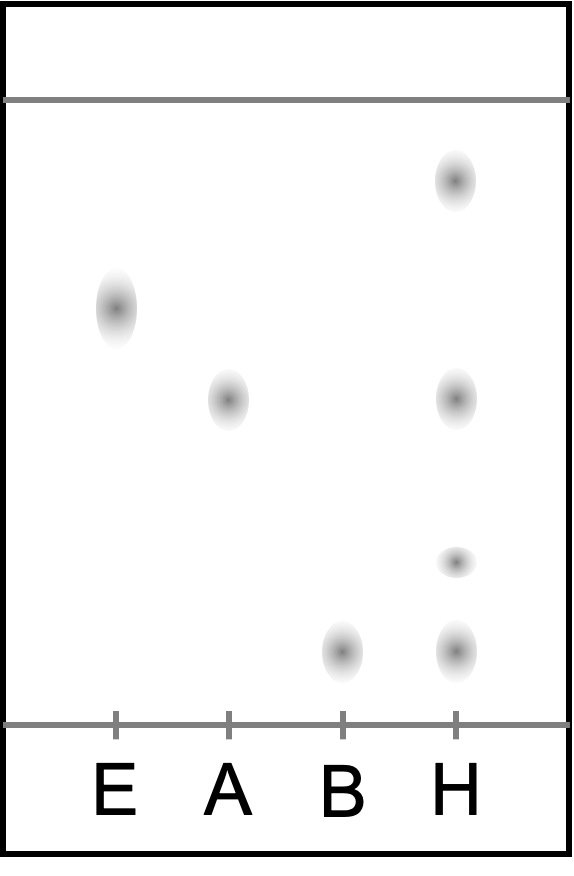
\includegraphics[scale=0.4]{../images/ccm_menthe.png}
\end{figure}
\end{enumerate}

\section*{Exercice 2 -- Acide fumarique ou maléique (6 points)}

L'acide fumarique et l'acide maléique ont la même formule chimique C\textsubscript{4}H\textsubscript{4}O\textsubscript{4}.
Le premier est utilisé comme additif alimentaire (c'est le E297) mais l'autre est nocif.
Il est donc essentiel de les identifier.

\begin{donnee}
\begin{center}
\begin{tabular}{l|c|c}
Espèce chimique & Acide fumarique & Acide maléique \\
\hline \hline
Température de fusion (\degree C) & 287 & 131 \\
Solubilité dans l'eau à 25\degree C (g/L) & 6{,}3 & 780 \\
Masse volumique (g/mL) & 1{,}64 & 1{,}59
\end{tabular}
\end{center}
La présence d'impuretés abaisse la température de fusion d'une espèce chimique solide.
Au contraire, si le solide n'est pas parfaitement sec, la température de fusion est augmentée.
\end{donnee}

\begin{enumerate}
\item \app{} Peut-on différencier expérimentalement l'acide maléique et l'acide fumarique par des mesures de masse volumique ?
Justifier.
\item Le banc Kofler est une plaque chauffante sur laquelle s'établit un gradient (une élévation régulière) de température.
Il permet la mesure de la température de fusion d'une espèce : on déplace le solide sur la plaque et on repère la température de fusion lorsque du liquide apparaît.
\begin{multicols}{2}
\begin{enumerate}
\item \app{} \rea{} \com{} La photographie ci-dessous montre le curseur lors d'une mesure de la température de fusion d'un échantillon inconnu : s'agit-il d'acide fumarique ou d'acide maléique ?
\item \val{} L'espèce déposée est-elle pure ?
\end{enumerate}

\center
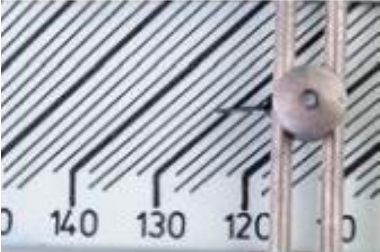
\includegraphics[scale=0.75]{../images/kofler_acide_maleique.png}
\end{multicols}
\end{enumerate}

\section*{Exercice 3 -- Sirop de menthe (7 points)}

Un élève souhaite connaitre la valeur de la masse volumique d'un sirop de menthe.
A l'aide d'une verrerie adaptée préalablement pesée (masse $m_0 = \unit{40{,}5}{\gram}$), il prélève un volume $V=\unit{9{,}7}{\milli\liter}$ de sirop.
Il pèse l'ensemble verrerie + sirop et lit sur la balance $m_\mathrm{tot} = \unit{53{,}6}{\gram}$.
\begin{enumerate}
\item \rco{} Rappeler la formule de la masse volumique, en précisant le nom et l'unité de chaque grandeur.
\item \anarai{} Établir la liste du matériel nécessaire pour que l'élève puisse réaliser la mesure.
\item \app{} \rea{} Quelle est la masse de sirop notée $m$ prélevée par l'élève ?
\item \rea{} En déduire la masse volumique du sirop de menthe, exprimée en kg/L.
\item \app{} Calculer la masse de sirop contenue dans une bouteille de 75\,cL.
\end{enumerate}
Sur l'étiquette de la bouteille, on peut lire : \og 70\,g de sucre pour 100\,g de sirop \fg{}.
\begin{figure}[h]
\center
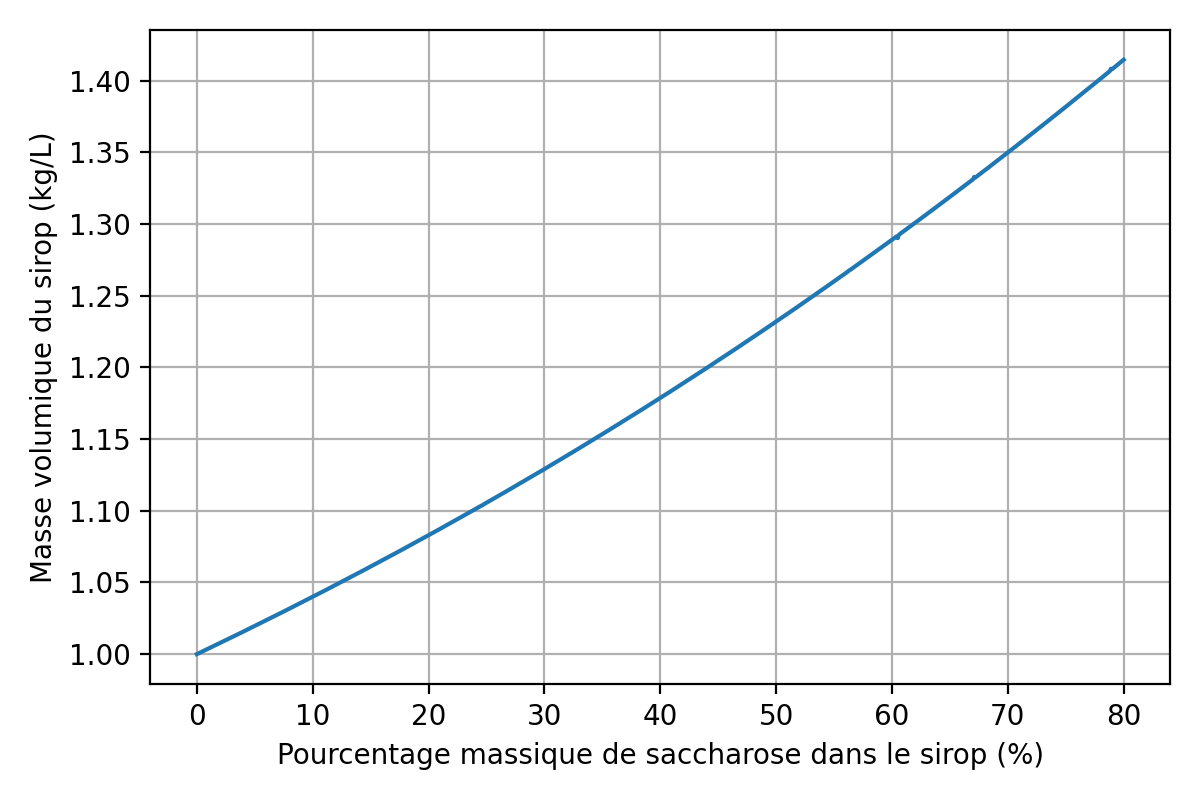
\includegraphics[scale=1]{../images/densite_sirop.png}
\caption{Évolution de la masse volumique d'un mélange d'eau et de sucre (saccharose) en fonction du pourcentage massique de saccharose dans le mélange.}
\label{fig:densite_sirop}
\end{figure}
\begin{enumerate}
\setcounter{enumi}{5}
\item \app{} \rea{} \val{} En vous aidant de la figure~\ref{fig:densite_sirop} ci-dessous, dire si la valeur trouvée précédemment est en accord avec les indications du fabricant.
Une construction graphique est attendue.
%\item \val{} (Bonus) En pesant la bouteille, on mesure 1{,}13\,kg.
%Proposer une explication à la différence entre cette valeur et la valeur mesurée précédemment.
\end{enumerate}

\end{document}


\section*{Exercice 4 -- Sirop de menthe (2) (10' -- 5 points)}

Un agent de la répression des fraudes souhaite vérifier que l'inscription \og Aux arômes naturels \fg{} inscrite sur la bouteille de sirop est vraie.
À l'usine de production, il prélève un échantillon de l'arôme utilisé pour le sirop et réalise une chromatographie sur couche mince (CCM).
Après avoir préparé une plaque de silice pour la CCM, il effectue quatre dépôts :
\begin{itemize}
\item l'arôme de menthe en S ;
\item du menthol en A ;
\item de la menthone en B ;
\item de l'huile essentielle de menthe poivrée en H, directement extraite de feuilles de menthe fraiche.
\end{itemize}
La plaque obtenue après élution et révélation est visible ci-dessous.
\begin{figure}[h]
\center
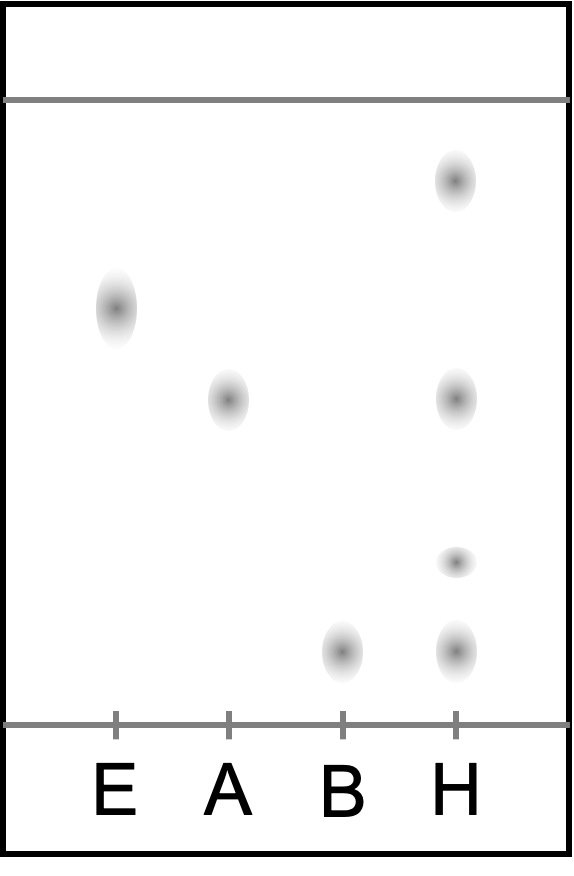
\includegraphics[scale=0.5]{../images/ccm_menthe.png}
\end{figure}

\begin{enumerate}
\item \rea{} D'après le chromatogramme ci-dessus, identifier les substances qui sont des corps purs et celles qui sont des mélanges.
\item \rea{} Y a-t-il de la menthone dans l'arôme du sirop ? Justifier.
\item \val{} L'agent décide d'interdire à la marque l'utilisation de l'inscription \og Aux arômes naturels \fg{}.
Justifier son choix.
\item \anarai{} Méfiant, il souhaite également vérifier que l'arôme n'est pas coupé à l'eau.
Proposer un protocole pour que l'agent puisse vérifier ses soupçons.
\end{enumerate}